\documentclass{article}
\usepackage{fullpage,amsmath,amsthm,graphicx,enumitem,amssymb}
\usepackage[hidelinks]{hyperref}
\usepackage{todonotes}
\usepackage{float}
\usepackage{tikz}
\usetikzlibrary{automata, positioning, arrows.meta, bending, decorations.pathmorphing}
\theoremstyle{definition}
\newtheorem{thm}{Theorem}
\newtheorem{question}[thm]{Question}
\newenvironment{solution}{\noindent\textit{Solution:}}{}

\newcommand{\reals}{\mathbb{R}}

\title{ASEN 5264 Decision Making under Uncertainty\\
       Homework 2: Markov Decision Processes}

\begin{document}

\maketitle

A submission should consist of two or three files:
\begin{itemize}[nosep]
    \item A single PDF file containing answers to questions (typed, handwritten, or exported notebook).
    \item JSON file output from \texttt{HW2.evaluate}.
    \item A code listing \emph{if the code is not included in the PDF}.
\end{itemize}

\section*{Conceptual Questions}

\begin{question}\label{q:q} (5 pts)
    \begin{enumerate}[label=\alph*)]
        \item Describe the difference between the reward function and the state-action {\color{purple}optimal} value function {\color{purple}($Q^*$)}.
        \item Write down an equation for the state-action {\color{purple}optimal} value in terms of $R$, $T$, and {\color{purple}$V^*$}.
    \end{enumerate}
\end{question}

\begin{question}\label{q:finite_mdp} (15 pts)
    Consider a game with 4 squares (enumerated 1-4 from left to right) in a horizontal line drawn on paper, a token, and a die. Each turn, the player can either roll the die or step to the next square. If the player rolls and the die shows an odd number, the token is moved one square to the right, and if an even number is rolled, the token is moved two squares to the right. The game ends when the token is on the 4th square. If the player steps when the token is on square 2, one point is subtracted; if the player steps when the token is on square 3, three points are added.
    \begin{figure}[H]
        \centering
        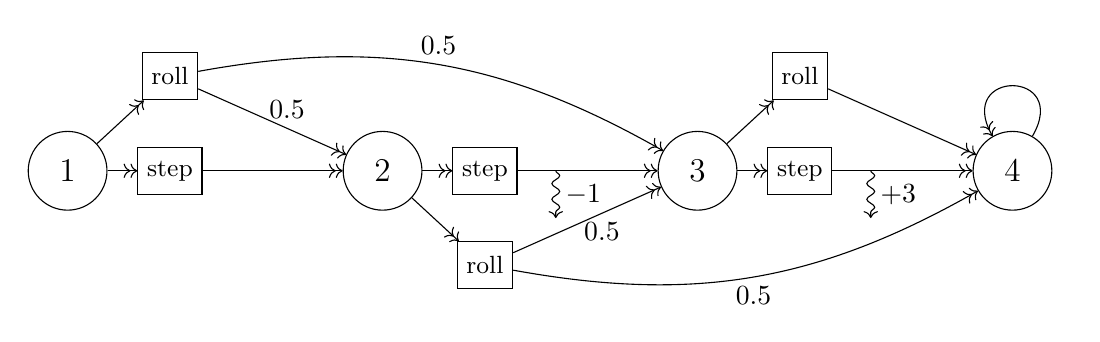
\begin{tikzpicture}[
            state/.style = {circle, draw, minimum size=1.0cm, font=\large},
            action/.style = {rectangle, draw, minimum size=0.6cm, font=\small},
            every edge/.style = {draw, thick},
            arr/.style = {->>},
        ]

            % States
            \node[state] (1) at (0,0) {$1$};
            \node[state] (2) at (4,0) {$2$};
            \node[state] (3) at (8,0) {$3$};
            \node[state] (4) at (12,0) {$4$};

            % Step actions (inline between states)
            \node[action] (step1) at (1.3,0) {step};
            \node[action] (step2) at (5.3,0) {step};
            \node[action] (step3) at (9.3,0) {step};

            % Roll actions (above/below)
            \node[action] (roll1) at (1.3,1.2) {roll};
            \node[action] (roll2) at (5.3,-1.2) {roll};
            \node[action] (roll3) at (9.3,1.2) {roll};

            % Step transitions
            \draw[->>] (1) -- (step1);
            \draw[->>] (step1) -- (2);
            \draw[->>] (2) -- (step2);
            \draw[->>] (step2) -- (3);
            \draw[->, decorate, decoration={snake, amplitude=0.5mm, segment length=2mm}] (6.2,0) -- node[right] {$-1$} ++(0,-0.6);
            \draw[->>] (3) -- (step3);
            \draw[->>] (step3) -- (4);
            \draw[->, decorate, decoration={snake, amplitude=0.5mm, segment length=2mm}] (10.2,0) -- node[right] {$+3$} ++(0,-0.6);

            % Roll transitions from state 1
            \draw[->>] (1) -- (roll1);
            \draw[->>] (roll1) -- node[above, pos=0.6] {0.5} (2);
            \draw[->>] (roll1) to[bend left=20] node[above] {0.5} (3);

            % Roll transitions from state 2
            \draw[->>] (2) -- (roll2);
            \draw[->>] (roll2) -- node[below, pos=0.6] {0.5} (3);
            \draw[->>] (roll2) to[bend right=20] node[below] {0.5} (4);

            % Roll transitions from state 3
            \draw[->>] (3) -- (roll3);
            \draw[->>] (roll3) -- (4);

            % Absorbing state loop
            \draw[->>] (4) to[out=60, in=120, looseness=5] (4);

        \end{tikzpicture}
    \end{figure}
    \begin{enumerate}[label=\alph*)]
        \item Formulate this problem as an MDP (write down $S$, $A$, $T$, and $R$).
        \item Use the Bellman backup algorithm to determine the optimal policy for this game, assuming a discount factor $\gamma = 0.95$?
    \end{enumerate}
\end{question}

\begin{question}\label{q:infinite_mdp} (15 pts)
    Consider a game with 3 squares in a horizontal line drawn on paper, a token, and a die. Each turn, the player can either reset or roll the die. {\color{purple}The token always starts in the leftmost square.} If the player rolls and the die shows an odd number, the token is moved one square to the right, and if an even number is rolled, the token is moved two squares to the right (in both cases stopping at the rightmost square\footnote{If the die is rolled from the middle square or right square, it will always end up in the right square.}). If the player resets, the token is always moved to the leftmost square. If the reset occurs when the token is in the middle square, two points are added; if the player resets when the token is on the right square, a point is subtracted.
    
%     \begin{figure}[H]
%         \centering
%         \begin{tikzpicture}[
%             > = Stealth,
%             node distance = 4cm,
%             on grid,
%             state/.style = {circle, draw, minimum size=1.0cm, font=\large},
%             every edge/.style = {draw, ->, >=Stealth, auto, bend left=20, thick},
%             every loop/.style = {looseness=4, thick, min distance=15mm}
%         ]
%         
%             % States
%             \node[state] (L) {$L$};
%             \node[state] (M) [right=of L] {$M$};
%             \node[state] (R) [right=of M] {$R$};
%         
%             % Roll actions from L
%             \path (L.180) edge[loop, in=120, out=60, looseness=5, min distance=15mm,] 
%             node[align=center, above=3mm] {reset} (L.179);
%             \path (L) edge[bend left=15] node[above=0mm] {roll: 0.5} (M);
%             \path (L) edge[bend left=30] node[above=0mm] {roll: 0.5} (R);
%         
%             % Roll actions from M
%             \path (M) edge[bend left=15] node[align=center, above=0mm] {reset: $r=+2$} (L);
%             \path (M) edge[bend left=15] node[above=0mm] {roll: $1$} (R);
%         
%             % Actions from R
%             \path (R) edge[bend left=30] node[align=center, below=2mm] {reset: $r = -1$} (L);
%             
%             % UPDATED LOOP POSITION
%             \path (R.359) edge[loop, in=300, out=240, looseness=5, min distance=15mm] 
%             node[align=center, right=0.1mm, below=1mm] {roll: $1$} (R.0);
%         
%             % Labels
%             \node[below=0.65cm of L] {\small Left};
%             \node[below=0.65cm of M] {\small Middle};
%             \node[below=0.65cm of R] {\small Right};
%         
%         \end{tikzpicture}
%     \end{figure}
    
    \begin{enumerate}[label=\alph*)]
        \item Formulate this problem as an MDP (write down $S$, $A$, $T$, and $R$). Assume a discount of $\gamma = 0.95$ {\color{purple}and that the die is fair}.
        \item Evaluate the following policy {\color{purple}assuming a fair die}:
        \begin{equation*}
            \pi(s) = \begin{cases}
                roll & \text{if } s = L \\
                reset & \text{if } s = M \\
                reset & \text{if } s = R
            \end{cases}
        \end{equation*}
        \item Suppose you are not sure that the die is fair (i.e. whether it will yield odd and even with equal probability). Give finite upper and lower bounds for the accumulated discounted score that you can expect to receive with discount $\gamma = 0.95$.
    \end{enumerate}
\end{question}

\section*{Exercise}

\begin{question} \label{q:gw}
    (Value iteration for Grid World, 35 pts)

    Solve the MDP \texttt{HW2.grid\_world} with your own implementation of value iteration with a discount of $\gamma=0.95$ and plot the resulting value function. All of the necessary information to solve this problem can be extracted with the \texttt{HW2.transition\_matrices} and \texttt{HW2.reward\_vectors} functions, and plotting can be accomplished with \texttt{\color{purple}POMDPTools.render(HW2.grid\_world, color=V)} where \texttt{v} is the value function. See the starter code and function docstrings for more information.
    {\color{red} FOR 2027: require submission of the plot.}
\end{question}

\section*{Challenge Problem}

\begin{question}\label{q:acas}
    (Value iteration for ACAS, 30 pts)

Your task is to find the optimal value function for an Aircraft Collision Avoidance System (ACAS). The encounter model will be specified as a Markov decision process, and your task will be to compute the value function for discount $\gamma=0.99$ using value iteration or another suitable algorithm that you implement. The continuous physical state space can be discretized at different levels of granularity, and the goal is to find the value function for the finest discretization possible.

A model with discretization level \texttt{n} can be constructed with
\begin{verbatim}
                        m = HW2.UnresponsiveACASMDP(n)
\end{verbatim}
The higher \texttt{n} is, the finer the discretization and the larger the state space. Again, all of the information needed to solve this problem can be extracted with the \texttt{HW2.transition\_matrices} and \texttt{HW2.reward\_vectors} functions, so you can start with your code from Question \ref{q:gw}.

The score received for solving the problem is \texttt{n}. You must submit your code for this problem along with the \texttt{results.json} file from executing \texttt{HW2.evaluate(v, "email@colorado.edu")} where \texttt{v} is the value function vector\footnote{\texttt{HW2.evaluate} will check the value function with a tolerance of $1 \times 10^{-6}$. However, the probabilities and rewards contain some small numbers, so results can vary slightly depending on the way these are added and multiplied. Therefore we recommend using a tolerance of $1 \times 10^{-8}$.}. A score of \texttt{n} = 7 or higher will receive full credit\footnote{Hints: If you run out of memory, consider using the \texttt{sparse} keyword argument mentioned in the docstring of \texttt{transition\_matrices}. By taking advantage of the structure of the problem, it is possible to attain a score of \texttt{n} = 20 with less than 10 minutes of computation time on a single core of a i7 laptop processor.}.

\end{question}

\end{document}
